%%%%%%%%%%%%%%%%%%%%%%%%%%%%%%%%%%%%%%%%%
% Journal Article
% LaTeX Template
% Version 1.4 (15/5/16)
%
% This template has been downloaded from:
% http://www.LaTeXTemplates.com
%
% Original author:
% Frits Wenneker (http://www.howtotex.com) with extensive modifications by
% Vel (vel@LaTeXTemplates.com)
%
% License:
% CC BY-NC-SA 3.0 (http://creativecommons.org/licenses/by-nc-sa/3.0/)
%
%%%%%%%%%%%%%%%%%%%%%%%%%%%%%%%%%%%%%%%%%

%----------------------------------------------------------------------------------------
%	PACKAGES AND OTHER DOCUMENT CONFIGURATIONS
%----------------------------------------------------------------------------------------

\documentclass[twoside,twocolumn]{article}

\usepackage{blindtext} % Package to generate dummy text throughout this template 

\usepackage[sc]{mathpazo} % Use the Palatino font
\usepackage[T1]{fontenc} % Use 8-bit encoding that has 256 glyphs
\linespread{1.05} % Line spacing - Palatino needs more space between lines
\usepackage{microtype} % Slightly tweak font spacing for aesthetics

\usepackage[english]{babel} % Language hyphenation and typographical rules

\usepackage[hmarginratio=1:1,top=32mm,columnsep=20pt]{geometry} % Document margins
\usepackage[hang, small,labelfont=bf,up,textfont=it,up]{caption} % Custom captions under/above floats in tables or figures
\usepackage{booktabs} % Horizontal rules in tables

\usepackage{lettrine} % The lettrine is the first enlarged letter at the beginning of the text

\usepackage{enumitem} % Customized lists
\setlist[itemize]{noitemsep} % Make itemize lists more compact

\usepackage{abstract} % Allows abstract customization
\renewcommand{\abstractnamefont}{\normalfont\bfseries} % Set the "Abstract" text to bold
\renewcommand{\abstracttextfont}{\normalfont\small\itshape} % Set the abstract itself to small italic text

\usepackage{titlesec} % Allows customization of titles
\renewcommand\thesection{\Roman{section}} % Roman numerals for the sections
\renewcommand\thesubsection{\roman{subsection}} % roman numerals for subsections
\titleformat{\section}[block]{\large\scshape\centering}{\thesection.}{1em}{} % Change the look of the section titles
\titleformat{\subsection}[block]{\large}{\thesubsection.}{1em}{} % Change the look of the section titles

\usepackage{fancyhdr} % Headers and footers
\pagestyle{fancy} % All pages have headers and footers
\fancyhead{} % Blank out the default header
\fancyfoot{} % Blank out the default footer
\fancyhead[C]{5584F $\bullet$ November 2019 $\bullet$ 4M20} % Custom header text
\fancyfoot[RO,LE]{\thepage} % Custom footer text

\usepackage{titling} % Customizing the title section

\usepackage{hyperref} % For hyperlinks in the PDF

\usepackage{graphicx}
\graphicspath{ {images/} }

\newenvironment{reusefigure}[2][htbp]
  {\addtocounter{figure}{-1}%
   \renewcommand{\theHfigure}{dupe-fig}% If you're using hyperref
   \renewcommand{\thefigure}{\ref{#2}}% Figure counter is \ref
   \renewcommand{\addcontentsline}[3]{}% Avoid placing figure in LoF
   \begin{figure}[#1]}
  {\end{figure}}
\usepackage{wrapfig}
\usepackage{amsmath}
\usepackage{xcolor}
\usepackage{listings}
\usepackage{subcaption}
\usepackage{pdfpages}
\usepackage{array,multirow,graphicx}
\lstset{
  basicstyle=\ttfamily,
  columns=fullflexible,
  frame=single,
  breaklines=true,
  postbreak=\mbox{\textcolor{red}{$\hookrightarrow$}\space},
}

\newcommand{\threepartdef}[6]
{
	\left\{
		\begin{array}{lll}
			#1 & \mbox{: } #2 \\
			#3 & \mbox{: } #4 \\
			#5 & \mbox{: } #6 \\
			0 & \mbox{: } otherwise
		\end{array}
	\right.
}
%----------------------------------------------------------------------------------------
%	TITLE SECTION
%----------------------------------------------------------------------------------------

\setlength{\droptitle}{-4\baselineskip} % Move the title up

\pretitle{\begin{center}\Huge\bfseries} % Article title formatting
\posttitle{\end{center}} % Article title closing formatting
\title{4M20 - Coursework One} % Article title
\author{%
\\
\textsc{Candidate Number: 5584F}% Your email address
}
\date{\today} % Leave empty to omit a date
\renewcommand{\maketitlehookd}{%
\begin{abstract}
\noindent
Three link robots are extremely versatile and can be used in applications ranging from robotic arms to moving robots. Throughout this investigation the three link robot was tasked with catching a ball at various trajectories. Kinematic control was considered for the majority of tasks due to the decreased complexity in computation compared to a dynamic model. The robot consists of three joints to move around 2D space, this creates lots of options for path trajectory, and robot shape. Planning algorithms were used to heuristically solve this problem to find a good solution quickly.
\end{abstract}
}
%----------------------------------------------------------------------------------------

\begin{document}
\onecolumn
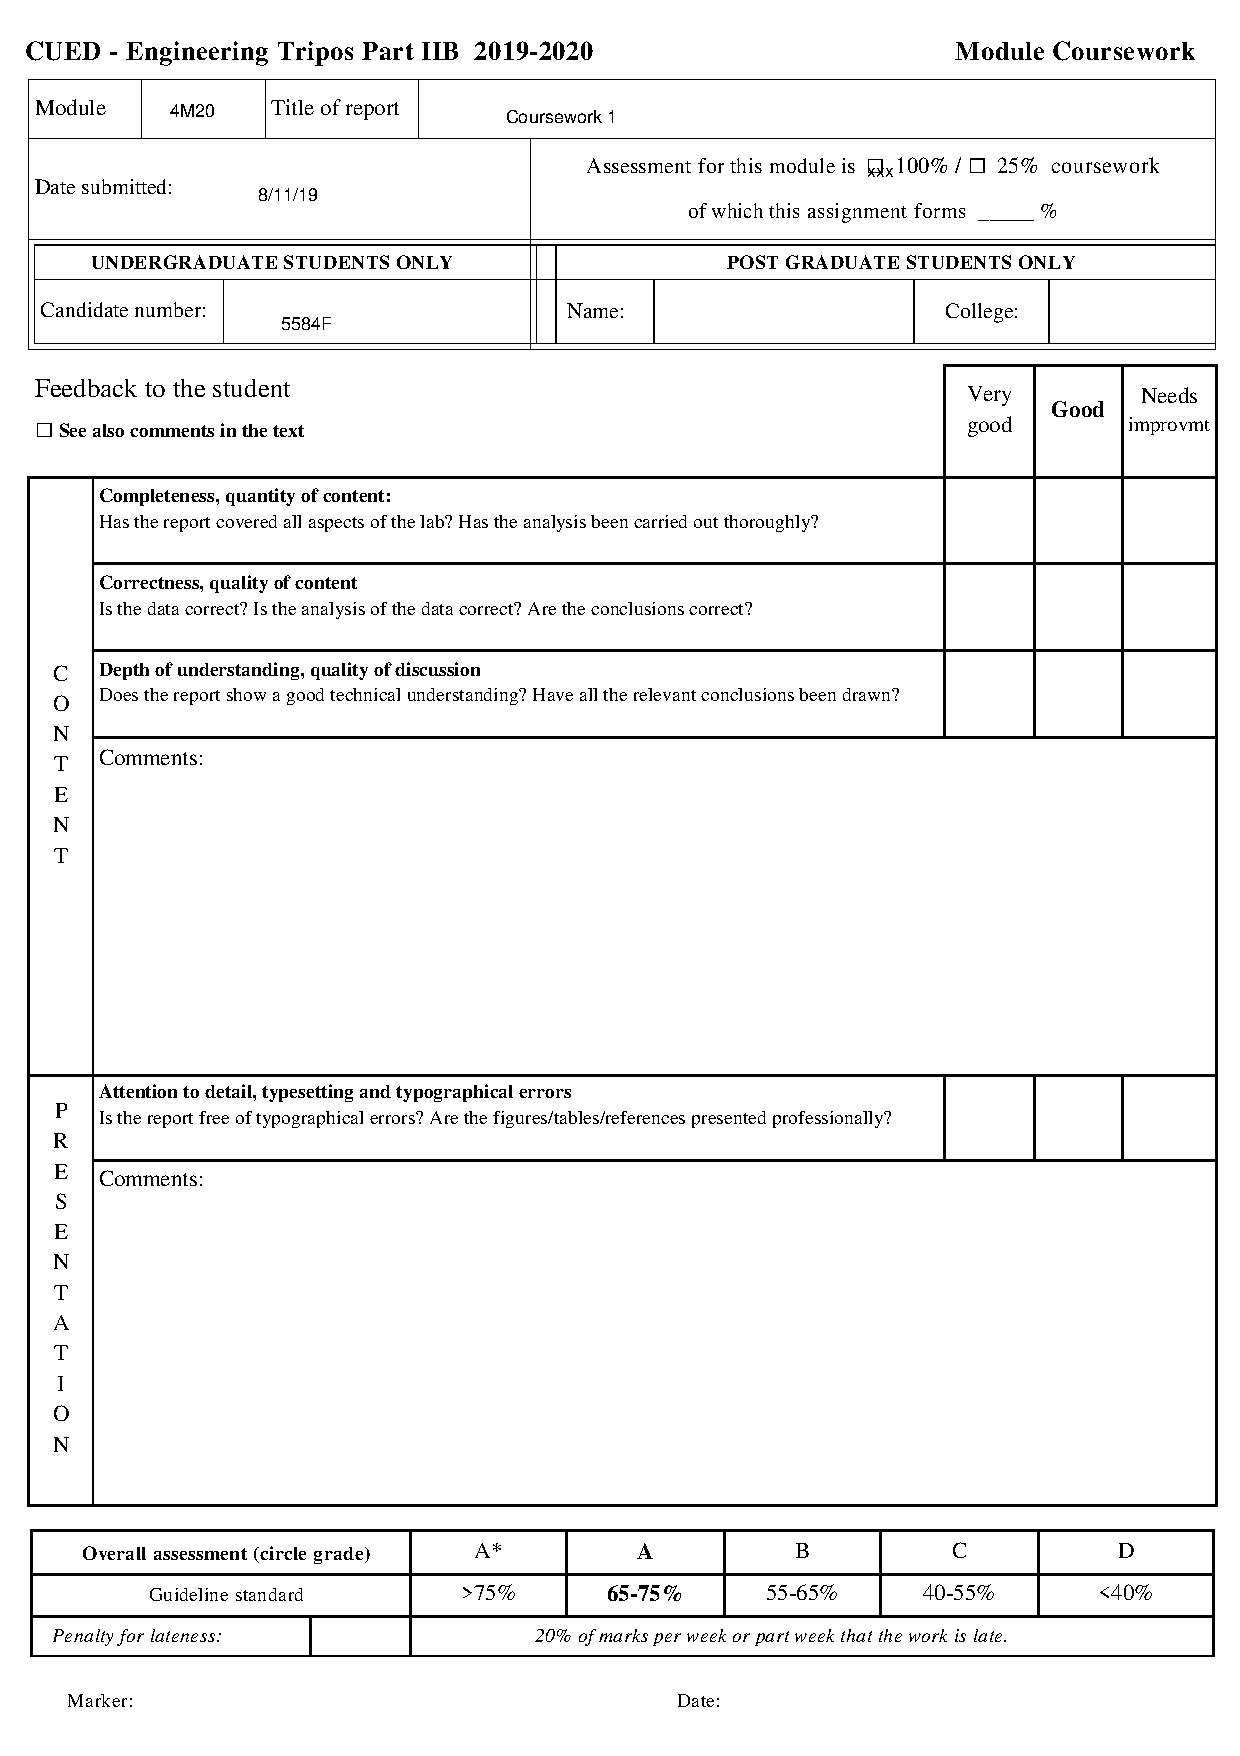
\includepdf[pages={1}]{coversheet.pdf}
\twocolumn
% Print the title
\maketitle

%----------------------------------------------------------------------------------------
%	ARTICLE CONTENTS
%----------------------------------------------------------------------------------------

\section{Introduction}

\lettrine[nindent=0em,lines=3]{T}heoretical and numeric investigations of a 3 link robotic manipulator are described in this report. The manipulator analysed is shown in \ref{fig:diagram} and is designed to catch a thrown ball. 

\begin{figure}[h]
  \centering
    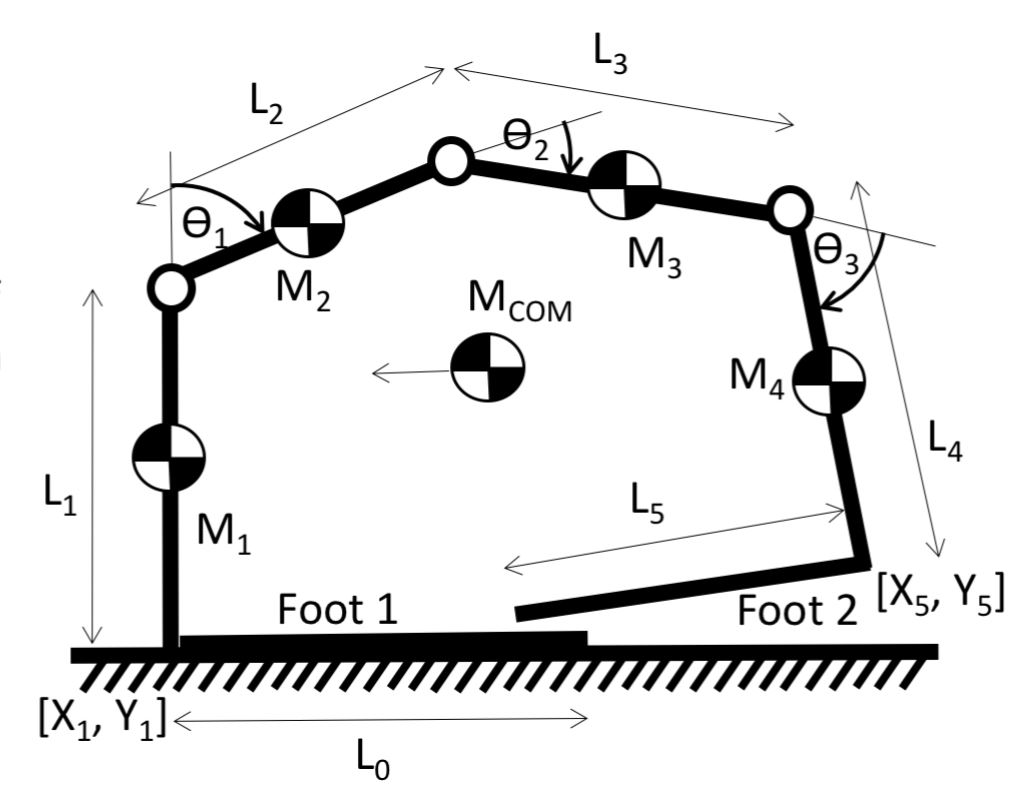
\includegraphics[width=\linewidth]{diagram}
  \caption{Diagram of robotic manipulator. L1=0.8m, L2=0.8m, L3=0.3m, $\theta1$=[-90,90], $\theta2$=[-160,160], $\theta3$=[-160,160]}
  \label{fig:diagram}
\end{figure}
%------------------------------------------------

\section{Question 1}
\subsection{Kinematic Control}
Kinematic control involves using the system geometry and knowledge of the world without sensing to build a desired motion through time. This motion defines the joint positions in our task. Kinematic control doesn't take forces or accelerations into account. This simplification reduces the complexity of the task drastically and allows for efficient planning methods to be implemented.
\newline
Two key aspects of kinematic control are forward kinematics, and inverse kinematics. In forward kinematics the manipulator joint angles $\boldsymbol{\theta}$ are used to calculate end effector position. The reverse occurs during inverse kinematics. In our case there are three control angles, and only two position co-ordinates. This leads to multiple viable solutions to inverse kinematics, which the best is chosen using planning algorithms.
\subsection{Feasible Region}
\begin{figure}[h]
  \centering
    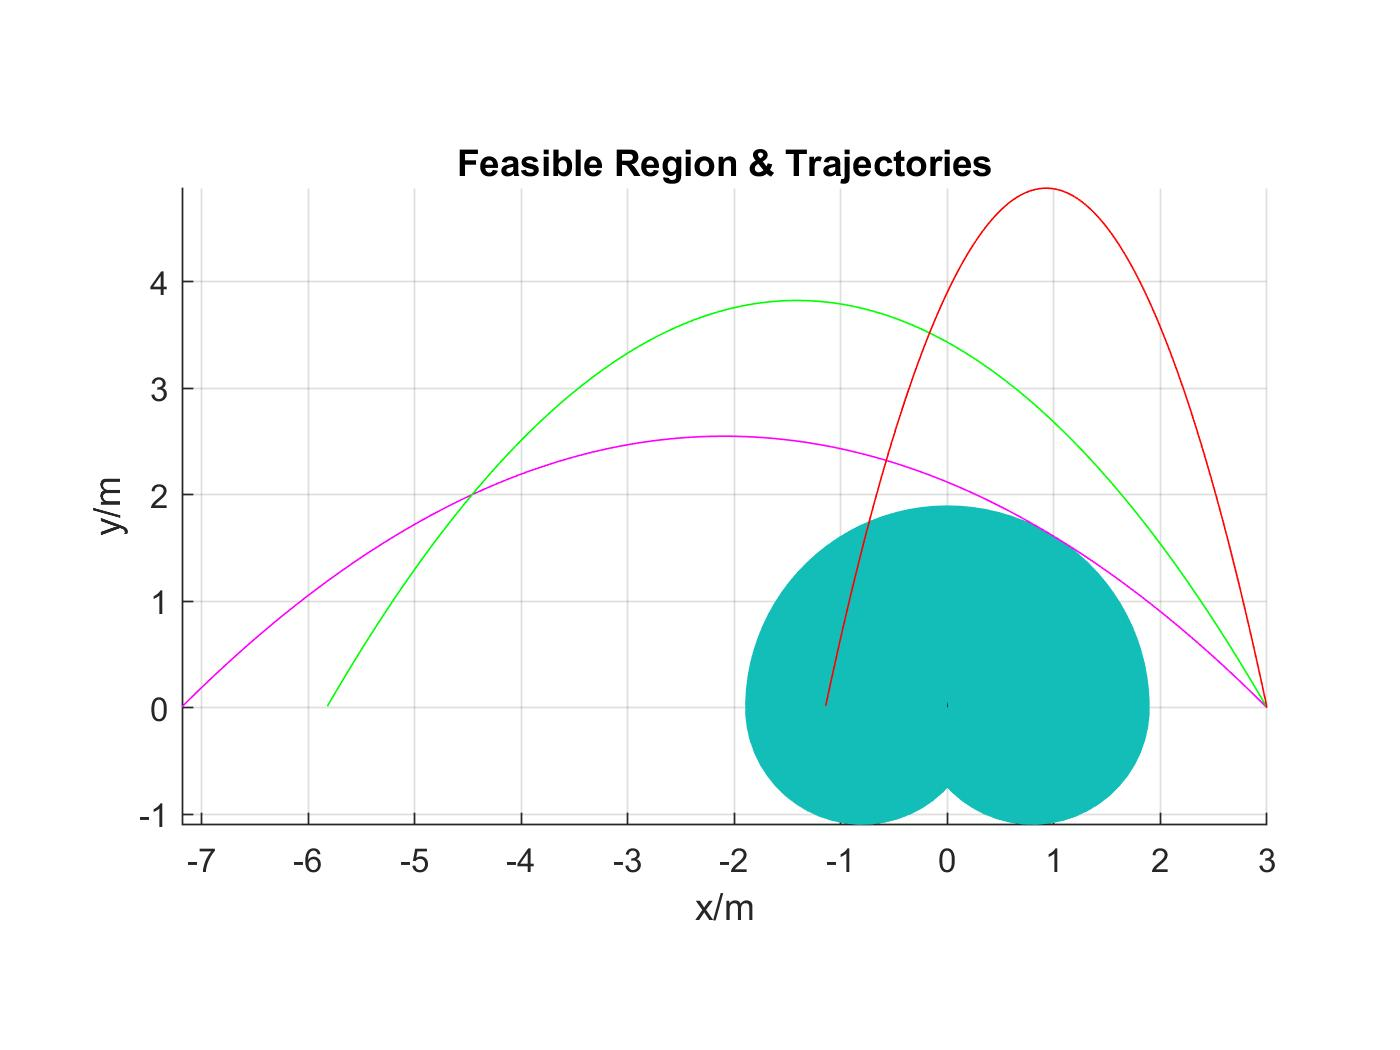
\includegraphics[width=\linewidth]{trajectory}
  \caption{Reachable range for the 3 link manipulator, ball trajectories are shown for questions 2 and 5}
  \label{fig:reachable_range}
\end{figure}

\subsection{Feasible Region}
\begin{figure}[h]
  \centering
    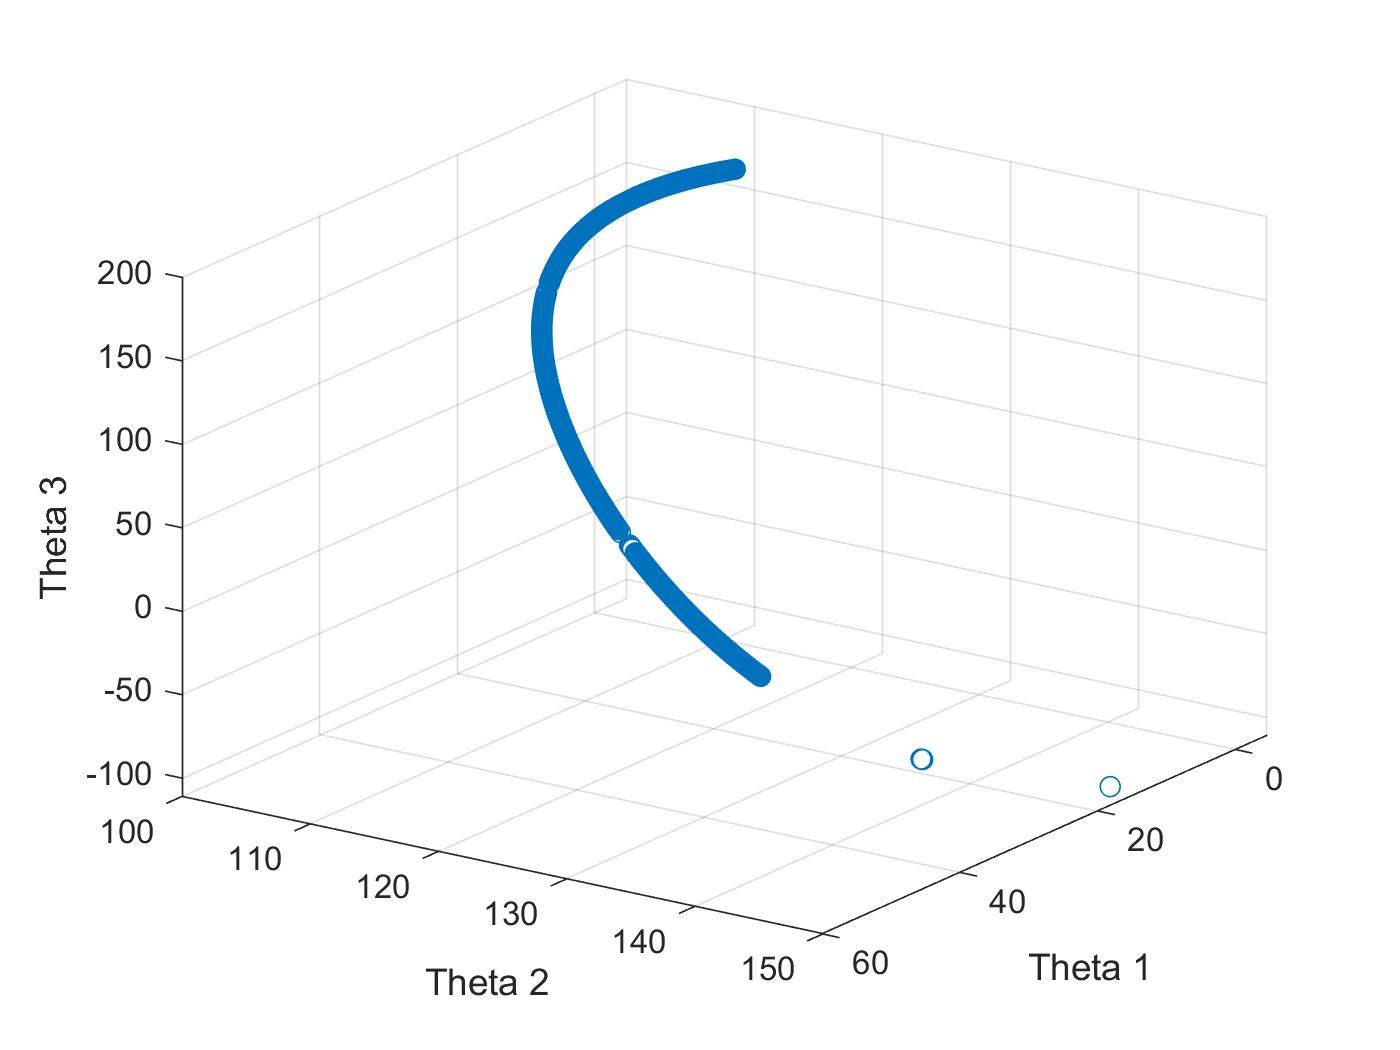
\includegraphics[width=\linewidth]{x=y=0-5}
  \caption{Viable joint angles to achieve x=y=0.5}
  \label{fig:sol}
\end{figure}

Figure \ref{fig:reachable_range} shows the reachable range for the robotic manipulator. With the constrains on angular position described in figure \ref{fig:diagram} this creates a semi circle region of radius 1.9m above y=0. The region below y=0 is also in accessible due to the floor, but is formed of two circles of radius 1.1m about [$\pm$0.8,0]. To calculate the feasible region the forward kinematics in equation \ref{eq:fk} were used and the variables were parametrically plotted. Different areas of the feasible region are accessible with differing combinations of joint angle, the region edge is only possible for one specific set of $\boldsymbol{\theta}$ for example.



To discover viable joint angles that result in [x,y]=[0.5,0.5] the inverse kinematics are required. However, our problem involves a redundant free variable not specified in the desired position. This variable is the end orientation and is $\theta_2+\theta_3-\theta_1$. This means that there will exist multiple curves of solutions that satisfy the end co-ordinates. Figure \ref{fig:sol} shows some of these solutions found by setting the desired orientation to lots of values. The solutions form a curved line, that signifies the intersection between the two complicated planes defined by the forward dynamics. Some of the solutions and resulting end co-ordinates are listed in table \ref{table:jointangle}. Figure \ref{fig:pos-1} visualises some of these possible positions.

\begin{figure}[h]
  \centering
    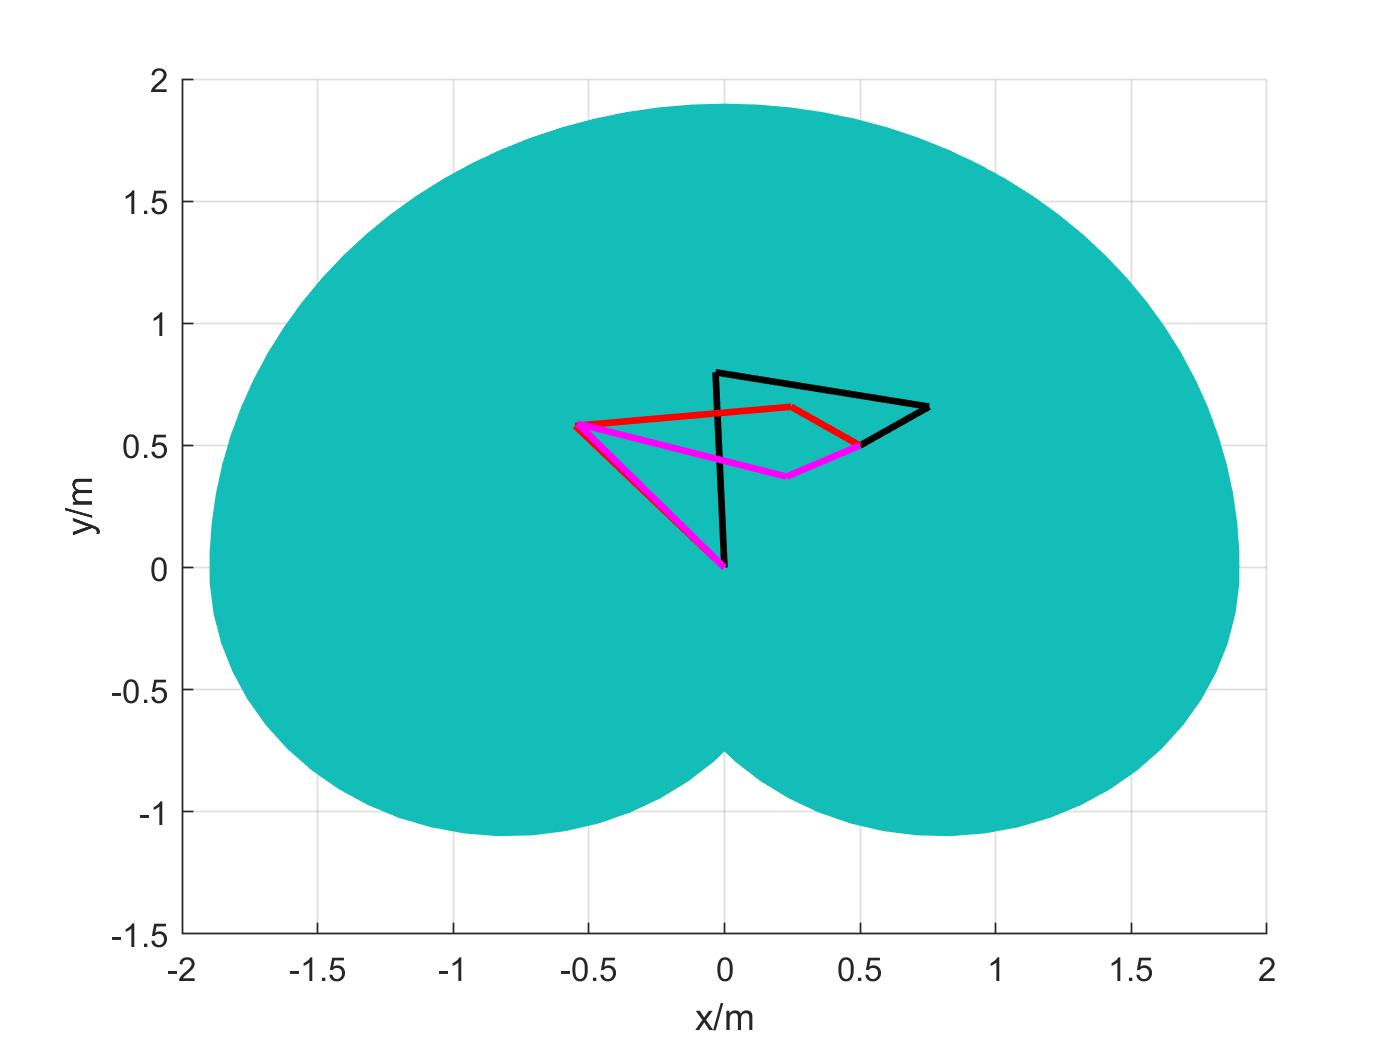
\includegraphics[width=\linewidth]{pos_1}
  \caption{Three possible joint angles that achieve x=y=0.5}
  \label{fig:pos-1}
\end{figure}


While each set of joint angles provides a valid solution to the positioning problem several factors make each solution more or less effective. This is down to factors such as required joint movement to reach end state, obstacles in trajectory, and required end orientation to catch ball. Throughout our problem no obstacles exist other then the floor which will never be in the way for a shot path so isn't considered. However, the minimisation of angle change will be considered. This directly effects both energy required and maximum required angular velocity. The $l_1$ norm of all required $\delta \boldsymbol{\theta} $  for the trajectory is compared to consider energy, or the $l_{\infty}$ norm for reducing maximum velocity.

\begin{table}[h]
\centering 
\begin{tabular}{ c | c | c | c | c }
$\theta_1$&$\theta_2$&$\theta_3$ & x & y \\ 

\midrule
2.377&102.5&137.9&0.4999&0.4998\\
43.49&127.9&37.63&0.4999&0.4992\\
42.58&148.3&-40.99&0.5001&0.5004\\
-0.1004&103.6&144.8&0.4995&0.5006\\
\end{tabular}
\caption{Some possible joint angles for [x,y]=[0.5,0.5]}
\label{table:jointangle}
\end{table}



%------------------------------------------------
\section{Question 2-3}
\subsection{Ball Dynamics}
For a ball thrown without drag equations \ref{eq:balldyn} can be used to generate the dynamics. The parameters take the values u=10m/s, $\alpha$=45, $x_0$=3m, $y_0$=0m, g=-9.81m/$s^2$. This is plotted in figure \ref{fig:reachable_range} and is shown to just clip the reachable range at between [x,y] = [1.09,1.55] and [0.85,1.69]. To catch the ball the end effector must be in the trajectory at the time of passing. Aim to meet the ball in the middle at [x,y]=[0.956,1.634]. the time the ball passes through is calculated using equation \ref{eq:balltime} and is 0.289s. 
\newline
The position of the end effector at this time is $\boldsymbol{\theta}$= [-25.65, 5.85, 8.256] , this is the solution that minimises $\Delta\boldsymbol{\theta}$ from the initial position. This solution was particularly easy to locate due to the end effectors close proximity to the feasible region edge, where $\theta_1, \theta_2$ are approximately 0. Figure \ref{fig:a=45} shows the possible solutions for this point and the chosen point that minimises the $l_1$ norm from the start position. Figure \ref{fig:caught} shows the final position of the arm.

\begin{figure}[h]
  \centering
    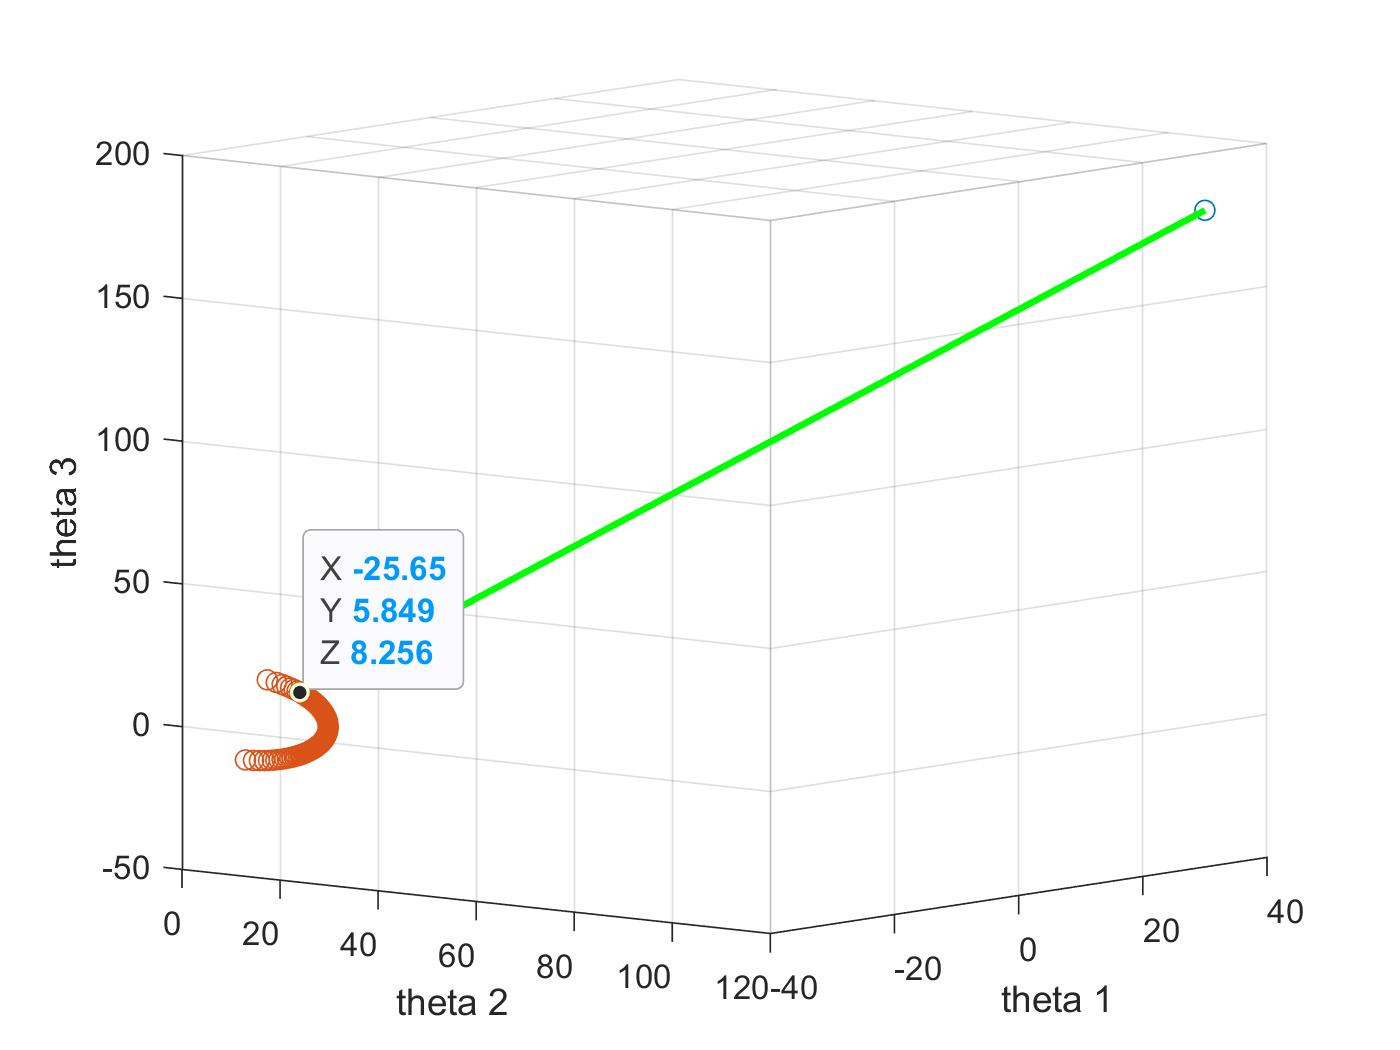
\includegraphics[width=\linewidth]{best_a=45}
  \caption{Optimised position to catch the ball thrown at 45 degrees}
  \label{fig:a=45}
\end{figure}

\begin{figure}[h]
  \centering
    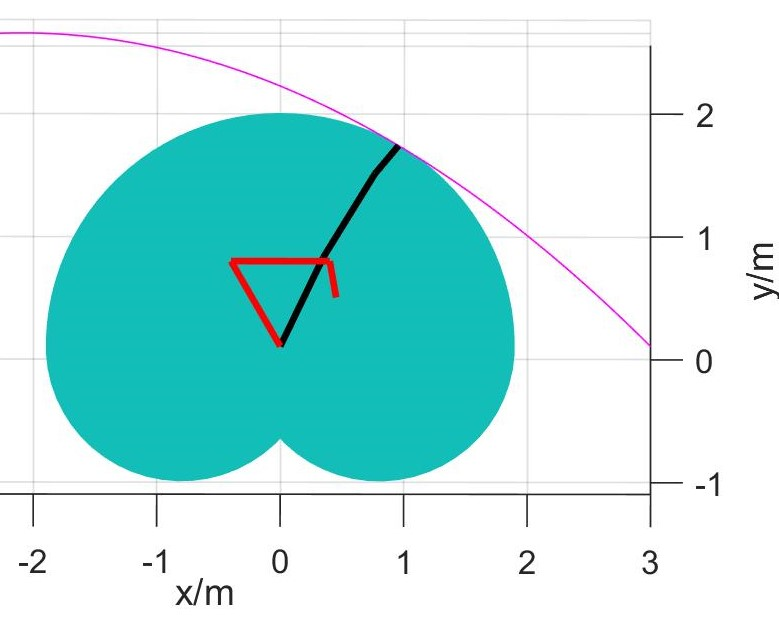
\includegraphics[width=\linewidth]{caughtball}
  \caption{Optimised position}
  \label{fig:caught}
\end{figure}

\begin{equation}
\begin{bmatrix}
x_b(t) \\
y_b(t)
\end{bmatrix}
=
\begin{bmatrix}
-uCos(\alpha)t+x_0\\
uSin(\alpha)t+0.5gt^2+y_0
\end{bmatrix}
\label{eq:balldyn}
\end{equation}

\begin{equation}
t= \frac{-uSin\alpha \pm \sqrt{u^2Sin^2\alpha+2gy}}{g}
\label{eq:balltime}
\end{equation}

\subsection{Joint Trajectories and Planning}
To calculate time series trajectories of joint angles the profile of angular speed must be considered. Figure \ref{fig:velp} shows multiple possible profiles. Each profile assumes zero velocity at the start and end, this might not be desirable if catching required matching the ball velocity. A step function is the ideal motion to evenly move the joint. However, in practice this is impossible due to the instantaneous change in speed and acceleration delta function. To fix this third or higher order polynomial functions could be implemented. These functions guarantee smooth accelerations and velocities but they don't take into account the physical limits of motors. A trapezoid function (smoothed in real application) is therefore used to represent the movement. Figure \ref{fig:velp} shows this velocity profile with two parameters $V_{max}$ and $a_{max}$ these are set by the motors used. In order to reach the desired position to catch the ball the integral of the velocity profile must equal the required angular change of each joint.
\newline
The time series equations for the velocity profile are listed in equation \ref{eq:vpro} and shown for each angle in figure \ref{fig:velp}. The acceleration time was optimised to minimise the sum |$\ddot{\theta}_{max}T/2+\dot{\theta}_{max}$|. These optimised acceleration and velocity maxima are listed in table \ref{table:jointvel}. For true theoretical minima of $\dot{\theta}_{max}$ and $\ddot{\theta}_{max}$ the velocity profiles are a step function, and triangular pulse respectively. If the arm can catch while moving then a ramp profile can be used to minimise acceleration further. The results for minimum $\dot{\theta}_{max}$ and $\ddot{\theta}_{max}$ for the step and ramp function can also be seen in table \ref{table:jointvel}.

\begin{table}[h]
\centering 
\begin{tabular}{ c | c | c }
Joint&|$\dot{\theta}_{max}$|&|$\ddot{\theta}_{max}$|\\ 

\midrule
1&303.9&2870\\
2&623.5&5888\\
3&391.8&3700\\
\midrule
1&192.6&$\infty$\\
2&395&$\infty$\\
3&248.2&$\infty$\\
\midrule
1&385&1333\\
2&790&2733\\
3&496&1718\\
\end{tabular}
\caption{Minimum |$\dot{\theta}_{max}$| and |$\ddot{\theta}_{max}$| when optimising a weighted sum, step function, and ramp function}
\label{table:jointvel}
\end{table}

\begin{figure*}[h]
\centering
    \begin{subfigure}[t]{0.33\linewidth}
        \centering
        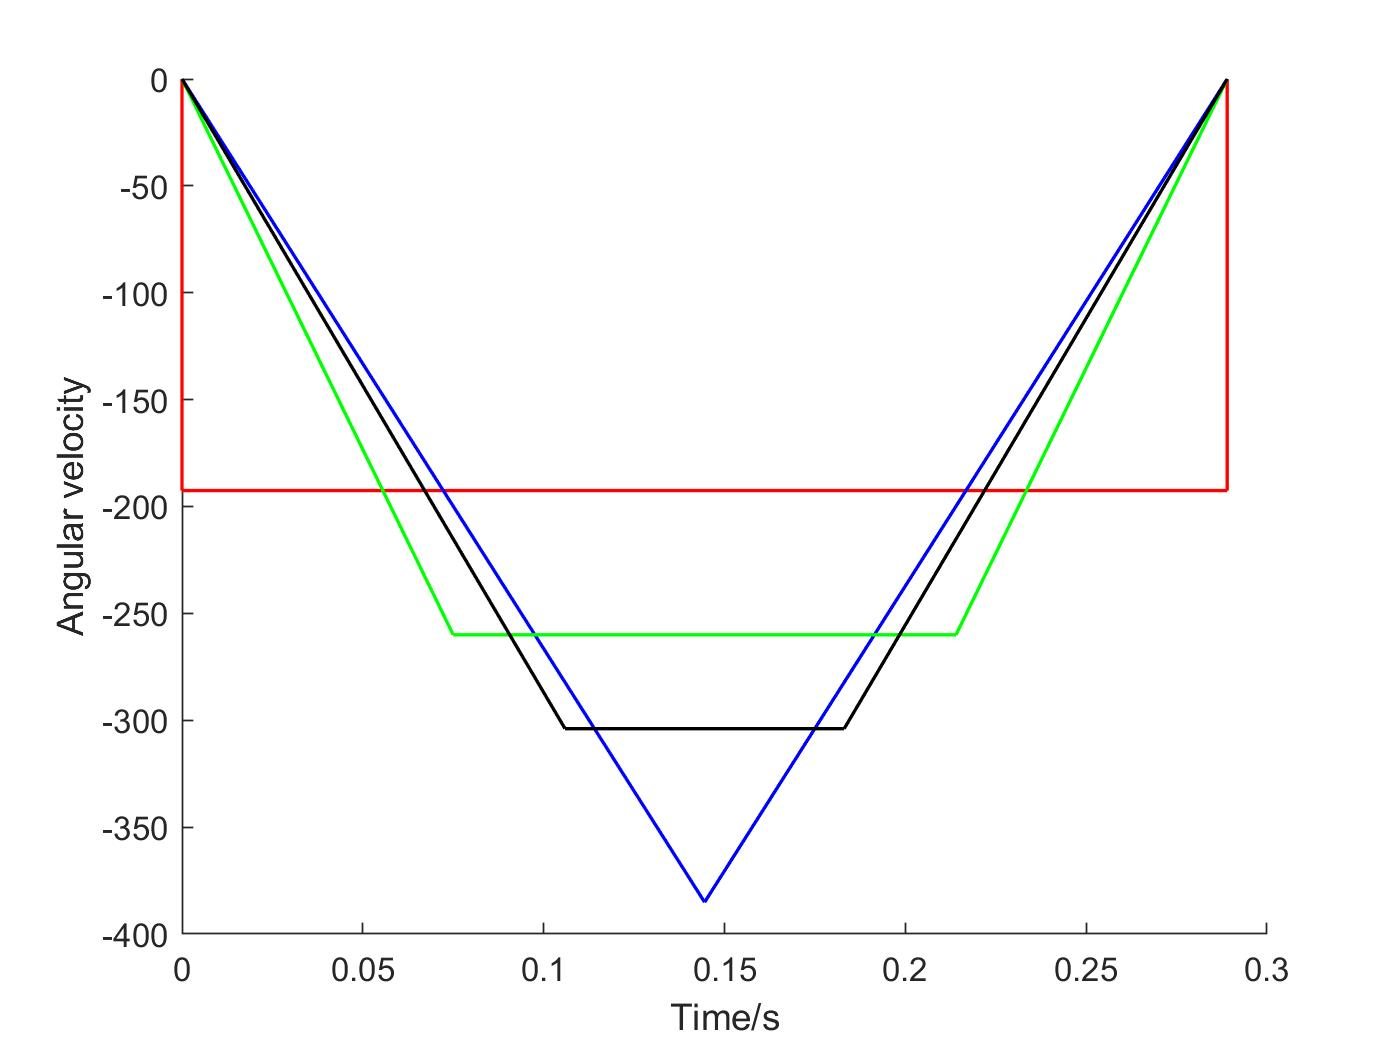
\includegraphics[width=\textwidth]{theta1}
        \caption{$\theta_1$}
        \label{sub:r1}
    \end{subfigure}%
    \begin{subfigure}[t]{0.33\linewidth}
        \centering
        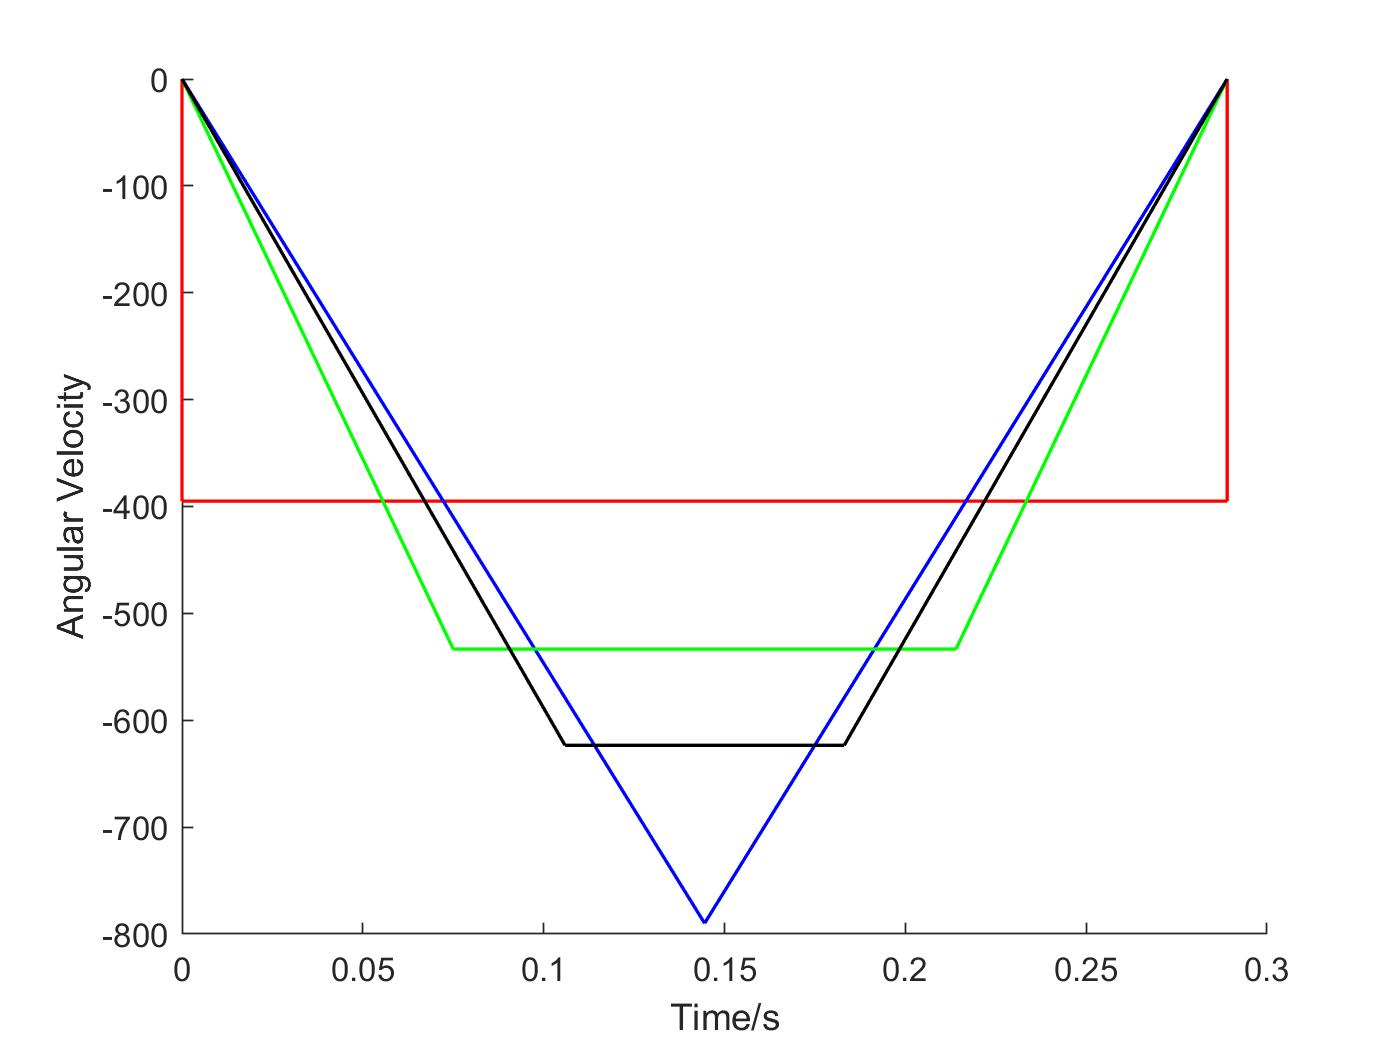
\includegraphics[width=\textwidth]{theta2}
        \caption{$\theta_2$ }
        \label{sub:r2}
    \end{subfigure}%
    \begin{subfigure}[t]{0.33\linewidth}
        \centering
        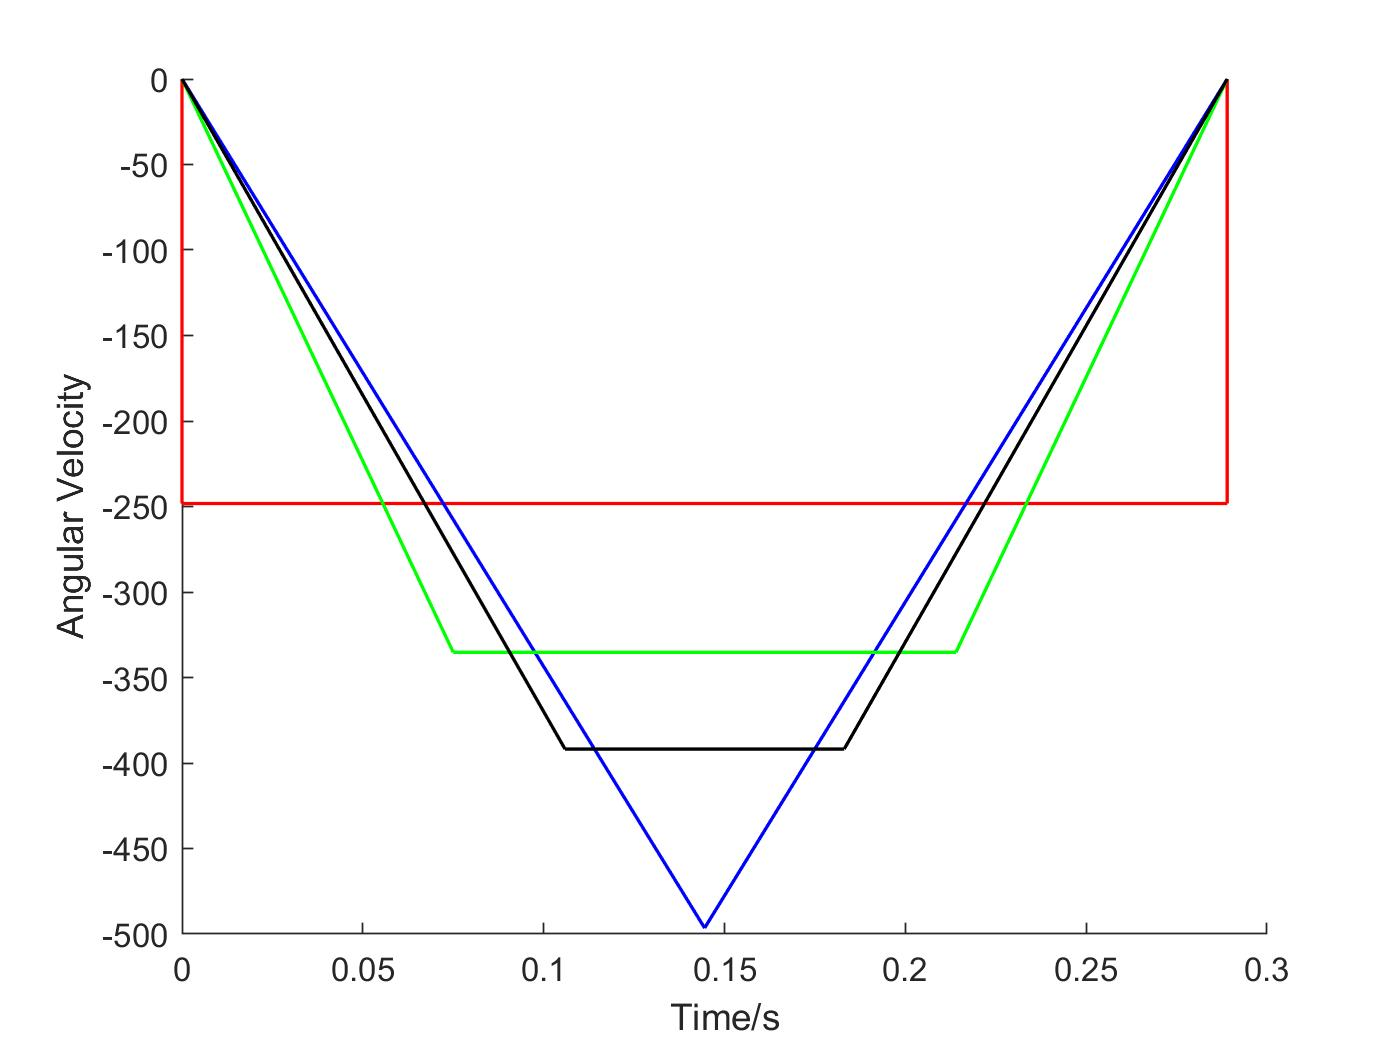
\includegraphics[width=\textwidth]{theta3}
        \caption{$\theta_3$ }
        \label{sub:r3}
    \end{subfigure}%
    \caption{Velocity profiles for each joint, red is the unit step, blue is minimising accelerations, green is an intermediate profile and black is optimised}
    \label{fig:velp}
\end{figure*}

\begin{equation}
\dot{\theta}_i = \threepartdef
{-\ddot{\theta}_{max}t     } 
{0<t<\frac{\dot{\theta}_{max}}{\ddot{\theta}_{max}}}
{\dot{\theta}_{max}}   
{
\frac{\dot{\theta}_{max}}{\ddot{\theta}_{max}} < t < T-\frac{\dot{\theta}_{max}}{\ddot{\theta}_{max}}}
{\ddot{\theta}_{max}(t-T) } 
{T-\frac{\dot{\theta}_{max}}{\ddot{\theta}_{max}}< t < T}
\label{eq:vpro}
\end{equation}
\newline
Another method of designing the angular time series is to first plan the end effector path. This can lead to minimising energy if for example the end effector is heavy, by taking the shortest route. This is achieved by dividing the desired path into small time steps and applying a trapezoid velocity profile to the path to allow smooth end movement. These small time steps result in required positions throughout time. This can be used in equation \ref{eq:inv} to calculate joint movement in time. This equation utilises the Jacobian which is seen in equation \ref{eq:jac}. In order to invert J($\boldsymbol{\theta}$) and determine angular movement the matrix must be square, this requires the addition of the end effector orientation ($\phi$). The orientation through time can be calculated to linearly change between start and end, or to fit other criteria in different tasks. 

\begin{equation}
\boldsymbol{\dot{\theta}}(t)=\boldsymbol{J(\theta)}^{-1}(\textbf{X}(t+1)-\textbf{X}(t)
\label{eq:inv}
\end{equation}




%------------------------------------------------
\section{Question 4}
\subsection{Dynamic Control} 
In dynamic control a model is build that uses forces and accelerations. For this to work we need to know the following:
\begin{itemize}
\item Mass and inertial matrix of each arm, link and the ball
\item Motor torques and accelerations 
\item Friction at joints
\item System latency
\end{itemize}
These are required so that the dynamics can be accurately modelled and turned into a time series to calculate the desired action and position.
As with kinematics there exists forward and inverse dynamics. The forward model takes the torques and forces and calculates robot trajectory. The inverse model reverses this and can be used to realise desired trajectories.
\newline
A kinematic model is far less complicated then a dynamic model due to these extra specifications that aren't required. This makes computation time and ease far better in a kinematic model. However, the extra complexity comes with the benefit of improved modelling and reaction to factors such as disturbances, balance and softening landings (ball catch or walking). Damping can be added to reach targets in a smooth way, without having to design a whole velocity profile as the dynamic model knows the extremes of the motors.

%------------------------------------------------------
\section{Question 5}
To catch a ball thrown at a variable angle a planning algorithm must occur. The algorithm helps to determine the required action to achieve the set goal. In order to know the goal and criteria for a good plan additional constrains must be applied to the problem.

\begin{itemize}
\item The ball must be caught within the feasible region, without bouncing
\item The ball must be caught at zero velocity
\item The path taken by the end effector should be minimised when locating the catching point
\item Planning algorithm should minimise joint velocity once a desired location has been found
\item Planning algorithm has knowledge of $\alpha$ and the thrown position
\end{itemize}



\begin{figure}[h]
  \centering
    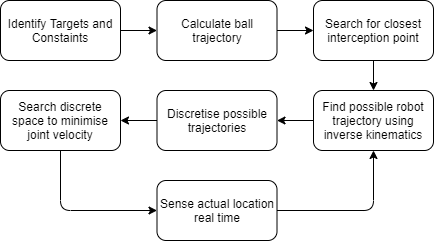
\includegraphics[width=\linewidth]{flowchart}
  \caption{Flow chart of discrete planning}
  \label{fig:flow}
\end{figure}

Figure \ref{fig:flow} shows a planning algorithm for catching the ball under these constants. This algorithm splits the problem into multiple optimisations for computational ease, this won't generate the best solution but will generate a good one. The first problem is locating the interception point, this can be done using an $l_2$ norm from the start position to the ball path. This can be analytically computed as there aren't multiple answers. The ball enters the feasible region when $\alpha$ =78 at 1.8s and hits the floor at 2s. The ball never enters the feasible region when $\alpha$=60 so the planning algorithm stops. Figure \ref{fig:reachable_range} shows these trajectories. The point on the trajectory that's closest to the start position of [x,y]=[0.4521 0.3974] from forward kinematics, is at [x,y]=[-0.9919,0.6986] the ball passes here at t=1.92s. Figure \ref{fig:bp} shows this optimum point.

\begin{figure}[h]
  \centering
    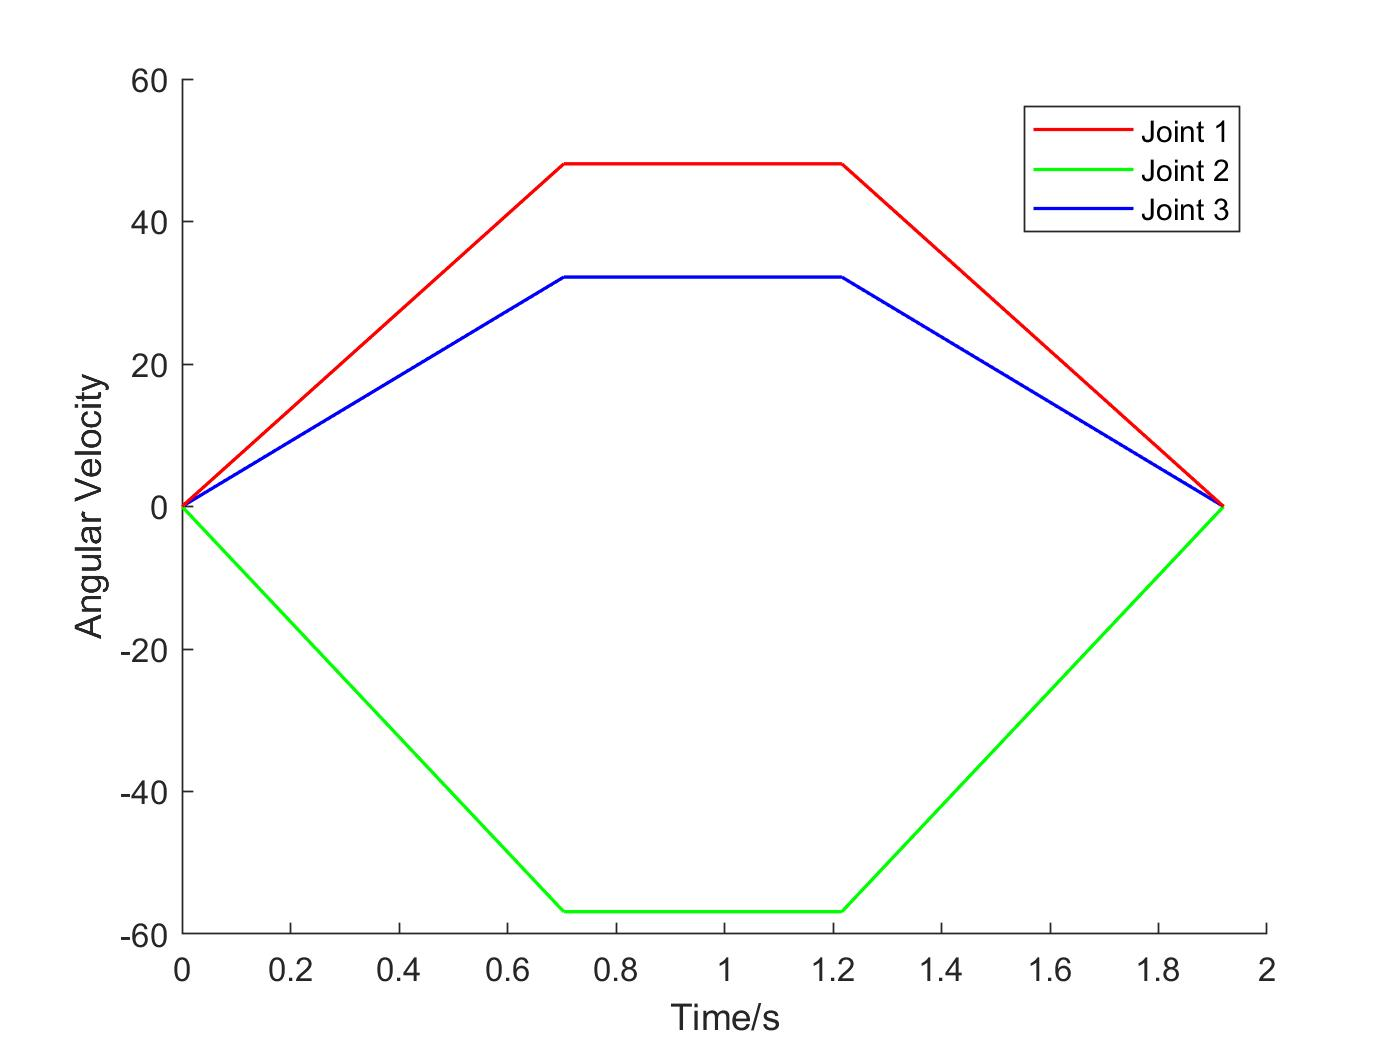
\includegraphics[width=\linewidth]{jointprofile}
  \caption{Velocity profile for the joins when minimising |$\dot{\theta}_{max}$| and |$\ddot{\theta}_{max}$|}
  \label{fig:bp}
\end{figure}
\begin{figure*}[h]
  \centering
    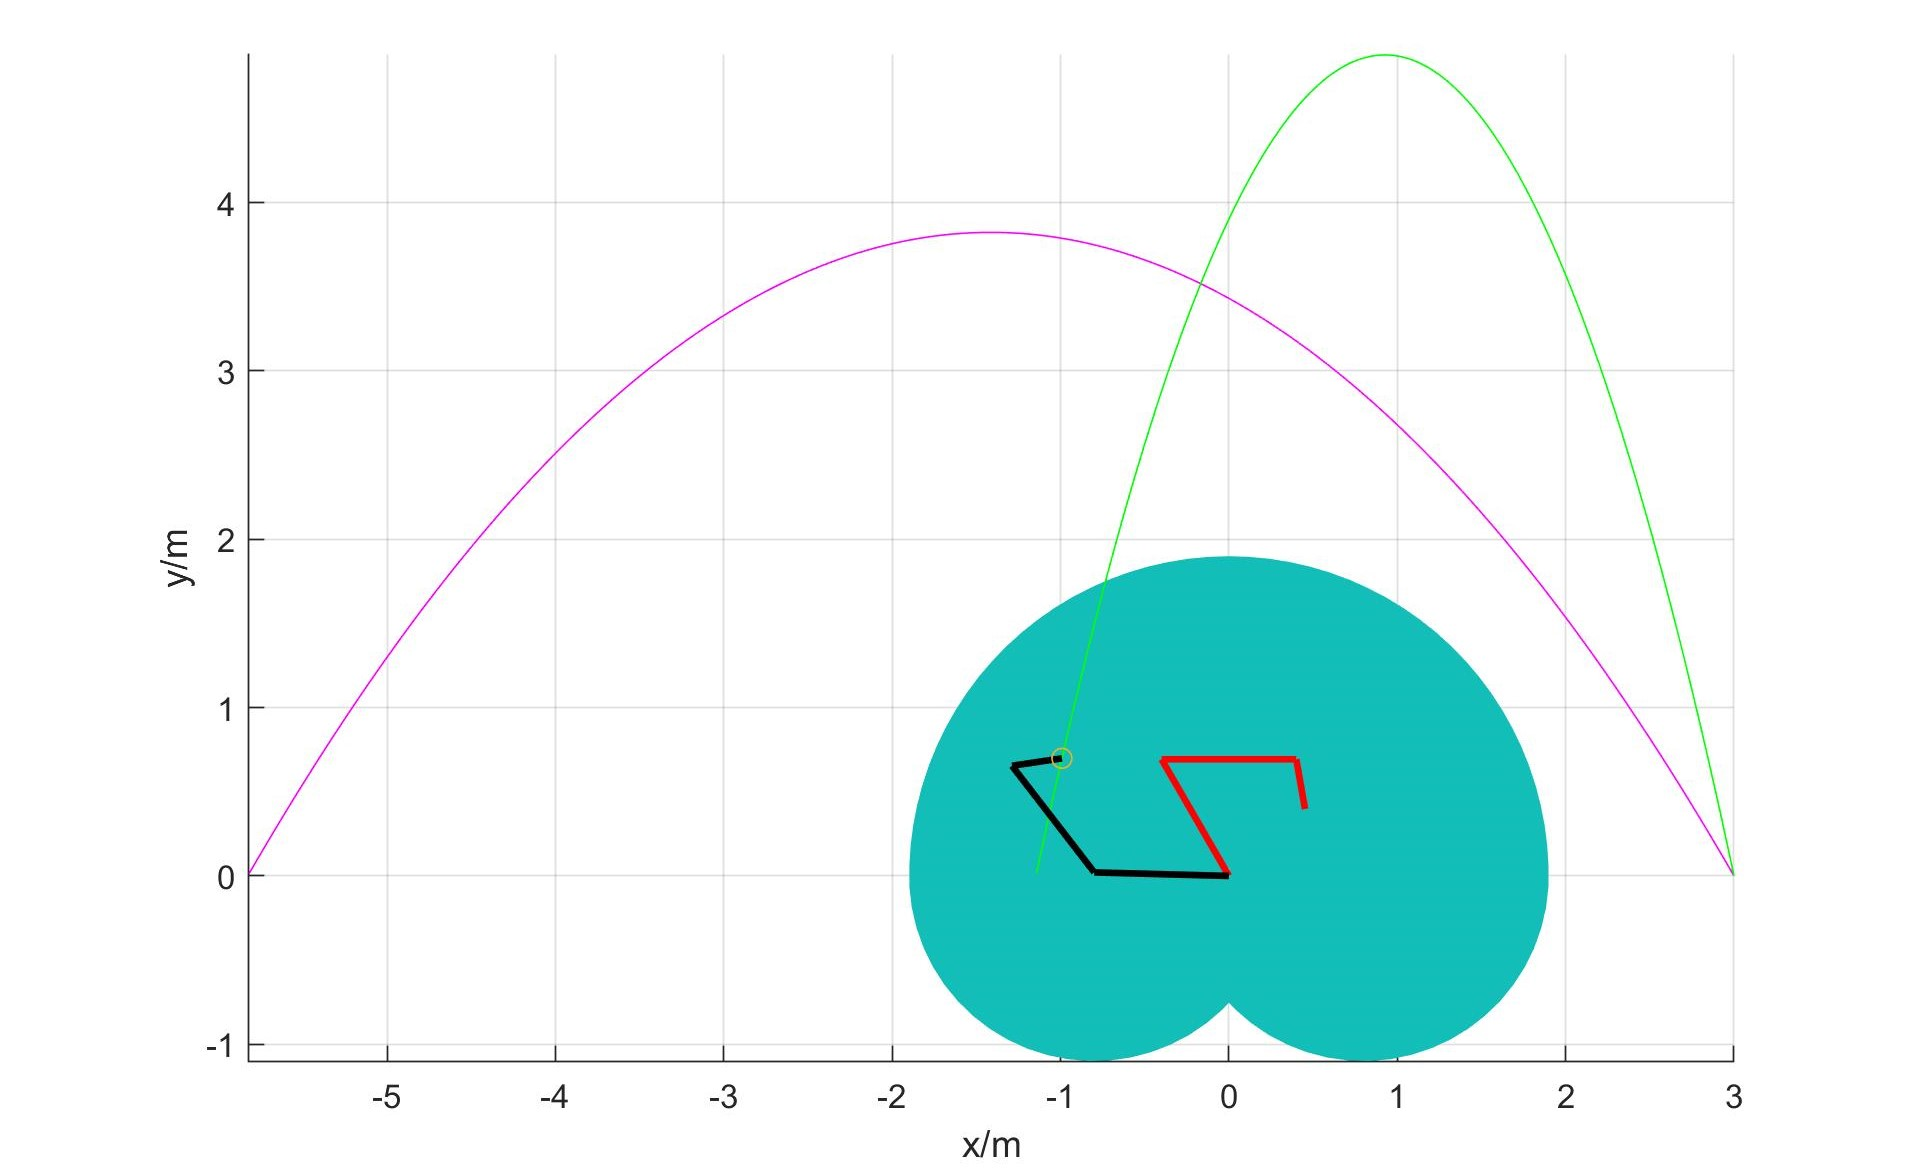
\includegraphics[width=\linewidth]{best_point}
  \caption{Closest location to catch ball}
  \label{fig:bp}
\end{figure*}

The next problem is to efficiently find a trajectory that minimises the join velocity. This can be done by assuming trapezoid velocity profiles for all the small discrete routes. Then for each small discrete step calculate the $l_{\infty}$ norm of the velocities, and choose the direction that minimises this. The search through discrete space can be done using a depth first search algorithm. Once all the steps have been optimised they can be combined to form the whole joint trajectory.
\newline
By discretionary the search space you greatly simplify the problem and reduce computation time, however it doesn't guarantee the best path as you cant move in all directions to find the direction of minimum joint velocity. 
\newline
The desired end position was found to be $\boldsymbol{\theta}$ =[88.4947,50.8256,119.1692] this can be seen in figure \ref{fig:bp}.
\newline
The time series trajectories of the joints follow equation \ref{eq:vpro} with $\boldsymbol{\dot{\theta}_{max}}$=[48.09,-56.87,32.2], $\boldsymbol{\ddot{\theta}_{max}}$=[68.33,-80.82,45.76], and T=1.92s.



\onecolumn
\section{Appendix}
\begin{equation}
\begin{bmatrix}
x \\
y
\end{bmatrix}
=
\begin{bmatrix}
-L_1Sin(\theta_1)+L_2Sin(\theta_2-\theta_1)+L_3Sin(\theta_2+\theta_3-\theta_1) \\
L_1Cos(\theta_1)+L_2Cos(\theta_2-\theta_1)+L_3Cos(\theta_2+\theta_3-\theta_1)
\end{bmatrix}
\label{eq:fk}
\end{equation}
 \begin{equation}
\boldsymbol{J(\theta)} = 
\begin{bmatrix}
-l_1cos(\theta_1)-l_2cos(\theta_2-\theta_1)-l_3cos(\phi) & l_2cos(\theta_2-\theta_1)+l_3cos(\phi)& l_3cos(\phi) \\
-l_1sin(\theta_1)+l_2sin(\theta_2-\theta_1)+l_3sin(\phi)& -l_2sin(\theta_2-\theta_1)-l_3sin(\phi)& -l_3sin(\phi) \\
-1 &1 &1
\end{bmatrix}
\label{eq:jac}
\end{equation} 
\subsection{Code}
\begin{lstlisting}[language=matlab]
l1=0.8;
l2=0.8;
l3=0.3;

plot_region(l1,l2,l3);
alphas=[60,78]%,60,78];
trajectory(alphas);
% draw_position([2.377,102.5,137.9],l1,l2,l3,'k');
% draw_position([43.49,127.9,37.63],l1,l2,l3,'r');
% draw_position([42.58,148.3,-40.99],l1,l2,l3,'m');

% draw_position([-25.65,5.85,8.256],l1,l2,l3,'k');
draw_position([30,120,80],l1,l2,l3,'r');
draw_position([88.4947,50.8256,119.1692],l1,l2,l3,'k');

title('');
xlabel('x/m');
ylabel('y/m');
hold on
scatter3(-0.9919,0.6986,0)
function plot_region(l1,l2,l3)
    syms t1 t2
    for t3 = -160:10:160
        x=-l1*sind(t1)+l2*sind(-t1+t2)+l3*sind(-t1+t2+t3);
        y=l1*cosd(t1)+l2*cosd(-t1+t2)+l3*cosd(-t1+t2+t3);
        z=x*0;
        h=ezsurf(x,y,z,[-90,90,-160,160]);
        h.EdgeColor = 'none';
        hold on
    end
end


function trajectory(alphas)
    g= 9.81;
    u=10;
    x0=3;
    y0=0;
    colours=['m','g','r','k']
    syms t
    for i =1:length(alphas)
        hold on
        alpha=alphas(i)
        x=-u*cosd(alpha)*t+x0;
        y=u*sind(alpha)*t+0.5*-g*t^2+y0;
        h=ezplot(x,y,[0,2.037*sind(alpha)]);
        h.Color = colours(i)
    end
    title('Feasible Region & Trajectories');
    xlabel('x/m');
    ylabel('y/m');
    %legend('alpha=45','alpha=60','alpha=78');
end



function draw_position(t,l1,l2,l3,c)
  
    x1=-l1*sind(t(1));
    y1=l1*cosd(t(1));
    
    x2=-l1*sind(t(1))+l2*sind(-t(1)+t(2));
    y2=l1*cosd(t(1))+l2*cosd(-t(1)+t(2));
    
    x3=-l1*sind(t(1))+l2*sind(-t(1)+t(2))+l3*sind(-t(1)+t(2)+t(3));
    y3=l1*cosd(t(1))+l2*cosd(-t(1)+t(2))+l3*cosd(-t(1)+t(2)+t(3));

    line([0 x1],[0 y1],[0 0],'color',c,'LineWidth',2);
    line([x1 x2],[y1 y2],[0 0],'color',c,'LineWidth',2);
    line([x2 x3],[y2 y3],[0 0],'color',c,'LineWidth',2);
end
\end{lstlisting}

\begin{lstlisting}[language=matlab]
x0=-0.9919;
y0=0.6986;
l1=0.8;
l2=0.8;
l3=0.3;

xs(1)=0;
ys(1)=0;
zs(1)=0;

count=1;
for phi = 0:0.25:360

    syms x y z
    Eq1 = -l1*sind(x)+l2*sind(y-x)+l3*sind(y+z-x) == x0 ;
    Eq2 = l1*cosd(x)+l2*cosd(y-x)+l3*cosd(y+z-x) == y0 ;
    Eq3 = y + z - x == phi;

    result = vpasolve(Eq1,Eq2,Eq3);
    s = size(result.x);
    for sol = 1:s(1)
        tempx =result.x(sol);
        tempy =result.y(sol);
        tempz =result.z(sol);
        if abs(tempx)<= 90 & abs(tempy)<=160 & abs(tempz)<=160
            xs(count)=tempx;
            ys(count)=tempy;
            zs(count)=tempz;
            count=count+1
        end
        
    end  
end

scatter3(xs,ys,zs);
\end{lstlisting}
%------------------------------------------------
\end{document}
